
%% bare_conf.tex
%% V1.4b
%% 2015/08/26
%% by Michael Shell
%% See:
%% http://www.michaelshell.org/
%% for current contact information.
%%
%% This is a skeleton file demonstrating the use of IEEEtran.cls
%% (requires IEEEtran.cls version 1.8b or later) with an IEEE
%% conference paper.
%%
%% Support sites:
%% http://www.michaelshell.org/tex/ieeetran/
%% http://www.ctan.org/pkg/ieeetran
%% and
%% http://www.ieee.org/

%%*************************************************************************
%% Legal Notice:
%% This code is offered as-is without any warranty either expressed or
%% implied; without even the implied warranty of MERCHANTABILITY or
%% FITNESS FOR A PARTICULAR PURPOSE! 
%% User assumes all risk.
%% In no event shall the IEEE or any contributor to this code be liable for
%% any damages or losses, including, but not limited to, incidental,
%% consequential, or any other damages, resulting from the use or misuse
%% of any information contained here.
%%
%% All comments are the opinions of their respective authors and are not
%% necessarily endorsed by the IEEE.
%%
%% This work is distributed under the LaTeX Project Public License (LPPL)
%% ( http://www.latex-project.org/ ) version 1.3, and may be freely used,
%% distributed and modified. A copy of the LPPL, version 1.3, is included
%% in the base LaTeX documentation of all distributions of LaTeX released
%% 2003/12/01 or later.
%% Retain all contribution notices and credits.
%% ** Modified files should be clearly indicated as such, including  **
%% ** renaming them and changing author support contact information. **
%%*************************************************************************


% *** Authors should verify (and, if needed, correct) their LaTeX system  ***
% *** with the testflow diagnostic prior to trusting their LaTeX platform ***
% *** with production work. The IEEE's font choices and paper sizes can   ***
% *** trigger bugs that do not appear when using other class files.       ***                          ***
% The testflow support page is at:
% http://www.michaelshell.org/tex/testflow/



\documentclass[conference]{IEEEtran}
% Some Computer Society conferences also require the compsoc mode option,
% but others use the standard conference format.
%
% If IEEEtran.cls has not been installed into the LaTeX system files,
% manually specify the path to it like:
% \documentclass[conference]{../sty/IEEEtran}





% Some very useful LaTeX packages include:
% (uncomment the ones you want to load)


% *** MISC UTILITY PACKAGES ***
%
%\usepackage{ifpdf}
% Heiko Oberdiek's ifpdf.sty is very useful if you need conditional
% compilation based on whether the output is pdf or dvi.
% usage:
% \ifpdf
%   % pdf code
% \else
%   % dvi code
% \fi
% The latest version of ifpdf.sty can be obtained from:
% http://www.ctan.org/pkg/ifpdf
% Also, note that IEEEtran.cls V1.7 and later provides a builtin
% \ifCLASSINFOpdf conditional that works the same way.
% When switching from latex to pdflatex and vice-versa, the compiler may
% have to be run twice to clear warning/error messages.






% *** CITATION PACKAGES ***
%
%\usepackage{cite}
% cite.sty was written by Donald Arseneau
% V1.6 and later of IEEEtran pre-defines the format of the cite.sty package
% \cite{} output to follow that of the IEEE. Loading the cite package will
% result in citation numbers being automatically sorted and properly
% "compressed/ranged". e.g., [1], [9], [2], [7], [5], [6] without using
% cite.sty will become [1], [2], [5]--[7], [9] using cite.sty. cite.sty's
% \cite will automatically add leading space, if needed. Use cite.sty's
% noadjust option (cite.sty V3.8 and later) if you want to turn this off
% such as if a citation ever needs to be enclosed in parenthesis.
% cite.sty is already installed on most LaTeX systems. Be sure and use
% version 5.0 (2009-03-20) and later if using hyperref.sty.
% The latest version can be obtained at:
% http://www.ctan.org/pkg/cite
% The documentation is contained in the cite.sty file itself.






% *** GRAPHICS RELATED PACKAGES ***
%
\ifCLASSINFOpdf
  % \usepackage[pdftex]{graphicx}
  % declare the path(s) where your graphic files are
  % \graphicspath{{../pdf/}{../jpeg/}}
  % and their extensions so you won't have to specify these with
  % every instance of \includegraphics
  % \DeclareGraphicsExtensions{.pdf,.jpeg,.png}
\else
  % or other class option (dvipsone, dvipdf, if not using dvips). graphicx
  % will default to the driver specified in the system graphics.cfg if no
  % driver is specified.
  % \usepackage[dvips]{graphicx}
  % declare the path(s) where your graphic files are
  % \graphicspath{{../eps/}}
  % and their extensions so you won't have to specify these with
  % every instance of \includegraphics
  % \DeclareGraphicsExtensions{.eps}
\fi
% graphicx was written by David Carlisle and Sebastian Rahtz. It is
% required if you want graphics, photos, etc. graphicx.sty is already
% installed on most LaTeX systems. The latest version and documentation
% can be obtained at: 
% http://www.ctan.org/pkg/graphicx
% Another good source of documentation is "Using Imported Graphics in
% LaTeX2e" by Keith Reckdahl which can be found at:
% http://www.ctan.org/pkg/epslatex
%
% latex, and pdflatex in dvi mode, support graphics in encapsulated
% postscript (.eps) format. pdflatex in pdf mode supports graphics
% in .pdf, .jpeg, .png and .mps (metapost) formats. Users should ensure
% that all non-photo figures use a vector format (.eps, .pdf, .mps) and
% not a bitmapped formats (.jpeg, .png). The IEEE frowns on bitmapped formats
% which can result in "jaggedy"/blurry rendering of lines and letters as
% well as large increases in file sizes.
%
% You can find documentation about the pdfTeX application at:
% http://www.tug.org/applications/pdftex





% *** MATH PACKAGES ***
%
%\usepackage{amsmath}
% A popular package from the American Mathematical Society that provides
% many useful and powerful commands for dealing with mathematics.
%
% Note that the amsmath package sets \interdisplaylinepenalty to 10000
% thus preventing page breaks from occurring within multiline equations. Use:
%\interdisplaylinepenalty=2500
% after loading amsmath to restore such page breaks as IEEEtran.cls normally
% does. amsmath.sty is already installed on most LaTeX systems. The latest
% version and documentation can be obtained at:
% http://www.ctan.org/pkg/amsmath





% *** SPECIALIZED LIST PACKAGES ***
%
%\usepackage{algorithmic}
% algorithmic.sty was written by Peter Williams and Rogerio Brito.
% This package provides an algorithmic environment fo describing algorithms.
% You can use the algorithmic environment in-text or within a figure
% environment to provide for a floating algorithm. Do NOT use the algorithm
% floating environment provided by algorithm.sty (by the same authors) or
% algorithm2e.sty (by Christophe Fiorio) as the IEEE does not use dedicated
% algorithm float types and packages that provide these will not provide
% correct IEEE style captions. The latest version and documentation of
% algorithmic.sty can be obtained at:
% http://www.ctan.org/pkg/algorithms
% Also of interest may be the (relatively newer and more customizable)
% algorithmicx.sty package by Szasz Janos:
% http://www.ctan.org/pkg/algorithmicx




% *** ALIGNMENT PACKAGES ***
%
%\usepackage{array}
% Frank Mittelbach's and David Carlisle's array.sty patches and improves
% the standard LaTeX2e array and tabular environments to provide better
% appearance and additional user controls. As the default LaTeX2e table
% generation code is lacking to the point of almost being broken with
% respect to the quality of the end results, all users are strongly
% advised to use an enhanced (at the very least that provided by array.sty)
% set of table tools. array.sty is already installed on most systems. The
% latest version and documentation can be obtained at:
% http://www.ctan.org/pkg/array


% IEEEtran contains the IEEEeqnarray family of commands that can be used to
% generate multiline equations as well as matrices, tables, etc., of high
% quality.




% *** SUBFIGURE PACKAGES ***
%\ifCLASSOPTIONcompsoc
%  \usepackage[caption=false,font=normalsize,labelfont=sf,textfont=sf]{subfig}
%\else
%  \usepackage[caption=false,font=footnotesize]{subfig}
%\fi
% subfig.sty, written by Steven Douglas Cochran, is the modern replacement
% for subfigure.sty, the latter of which is no longer maintained and is
% incompatible with some LaTeX packages including fixltx2e. However,
% subfig.sty requires and automatically loads Axel Sommerfeldt's caption.sty
% which will override IEEEtran.cls' handling of captions and this will result
% in non-IEEE style figure/table captions. To prevent this problem, be sure
% and invoke subfig.sty's "caption=false" package option (available since
% subfig.sty version 1.3, 2005/06/28) as this is will preserve IEEEtran.cls
% handling of captions.
% Note that the Computer Society format requires a larger sans serif font
% than the serif footnote size font used in traditional IEEE formatting
% and thus the need to invoke different subfig.sty package options depending
% on whether compsoc mode has been enabled.
%
% The latest version and documentation of subfig.sty can be obtained at:
% http://www.ctan.org/pkg/subfig




% *** FLOAT PACKAGES ***
%
%\usepackage{fixltx2e}
% fixltx2e, the successor to the earlier fix2col.sty, was written by
% Frank Mittelbach and David Carlisle. This package corrects a few problems
% in the LaTeX2e kernel, the most notable of which is that in current
% LaTeX2e releases, the ordering of single and double column floats is not
% guaranteed to be preserved. Thus, an unpatched LaTeX2e can allow a
% single column figure to be placed prior to an earlier double column
% figure.
% Be aware that LaTeX2e kernels dated 2015 and later have fixltx2e.sty's
% corrections already built into the system in which case a warning will
% be issued if an attempt is made to load fixltx2e.sty as it is no longer
% needed.
% The latest version and documentation can be found at:
% http://www.ctan.org/pkg/fixltx2e


%\usepackage{stfloats}
% stfloats.sty was written by Sigitas Tolusis. This package gives LaTeX2e
% the ability to do double column floats at the bottom of the page as well
% as the top. (e.g., "\begin{figure*}[!b]" is not normally possible in
% LaTeX2e). It also provides a command:
%\fnbelowfloat
% to enable the placement of footnotes below bottom floats (the standard
% LaTeX2e kernel puts them above bottom floats). This is an invasive package
% which rewrites many portions of the LaTeX2e float routines. It may not work
% with other packages that modify the LaTeX2e float routines. The latest
% version and documentation can be obtained at:
% http://www.ctan.org/pkg/stfloats
% Do not use the stfloats baselinefloat ability as the IEEE does not allow
% \baselineskip to stretch. Authors submitting work to the IEEE should note
% that the IEEE rarely uses double column equations and that authors should try
% to avoid such use. Do not be tempted to use the cuted.sty or midfloat.sty
% packages (also by Sigitas Tolusis) as the IEEE does not format its papers in
% such ways.
% Do not attempt to use stfloats with fixltx2e as they are incompatible.
% Instead, use Morten Hogholm'a dblfloatfix which combines the features
% of both fixltx2e and stfloats:
%
% \usepackage{dblfloatfix}
% The latest version can be found at:
% http://www.ctan.org/pkg/dblfloatfix




% *** PDF, URL AND HYPERLINK PACKAGES ***
%
%\usepackage{url}
% url.sty was written by Donald Arseneau. It provides better support for
% handling and breaking URLs. url.sty is already installed on most LaTeX
% systems. The latest version and documentation can be obtained at:
% http://www.ctan.org/pkg/url
% Basically, \url{my_url_here}.




% *** Do not adjust lengths that control margins, column widths, etc. ***
% *** Do not use packages that alter fonts (such as pslatex).         ***
% There should be no need to do such things with IEEEtran.cls V1.6 and later.
% (Unless specifically asked to do so by the journal or conference you plan
% to submit to, of course. )


% correct bad hyphenation here
\hyphenation{op-tical net-works semi-conduc-tor}

\usepackage{setspace}
\usepackage{geometry}
\geometry{left=1in,right=1in,top=1in,bottom=1in}
\usepackage{graphics}
\usepackage{algorithmic}
\usepackage{algorithm}
\usepackage{epsfig}

\newtheorem{THM}{Theorem}[section]
\newtheorem{COR}{Corrolary}[section]
\newtheorem{PRF}{Proof}
\newtheorem{DEF}{Definition}[section]


\begin{document}
%
% paper title
% Titles are generally capitalized except for words such as a, an, and, as,
% at, but, by, for, in, nor, of, on, or, the, to and up, which are usually
% not capitalized unless they are the first or last word of the title.
% Linebreaks \\ can be used within to get better formatting as desired.
% Do not put math or special symbols in the title.
\title{Towards a Decision Support System by the\\ study of Cell malfunctions for Breast Cancer}


% author names and affiliations
% use a multiple column layout for up to three different
% affiliations


\author{\IEEEauthorblockN{ Sampurna Mandal, Supratim Bhattacharya, and Jayanta Poray}
\IEEEauthorblockA{Department of Computer Science \& Engineering\\
Techno India University, West Bengal\\
EM\ /1 -  Salt Lake, Sector - V, Kolkata - 91, INDIA\\
Email: piu.sampurna@gmail.com, bhattacharya.supratim@gmail.com,  jayanta.poray@gmail.com}}
%\and
%\IEEEauthorblockN{Sampurna Mandal}
%\IEEEauthorblockA{Department of Computer\\Science \& Engineering\\
%Techno India University\\
%EM\ /1 -  Salt Lake, Sector - V\\ Kolkata - 91, West Bengal, INDIA\\
%Email: piu.sampurna@gmail.com }
%\and
%\IEEEauthorblockN{James}
%\IEEEauthorblockA{Starfleet Academy\\
%San Francisco, California 96678--2391\\
%Telephone: (800) 555--1212\\
%Fax: (888) 555--1212}}

% conference papers do not typically use \thanks and this command
% is locked out in conference mode. If really needed, such as for
% the acknowledgment of grants, issue a \IEEEoverridecommandlockouts
% after \documentclass

% for over three affiliations, or if they all won't fit within the width
% of the page, use this alternative format:
% 
%\author{\IEEEauthorblockN{Michael Shell\IEEEauthorrefmark{1},
%Homer Simpson\IEEEauthorrefmark{2},
%James Kirk\IEEEauthorrefmark{3}, 
%Montgomery Scott\IEEEauthorrefmark{3} and
%Eldon Tyrell\IEEEauthorrefmark{4}}
%\IEEEauthorblockA{\IEEEauthorrefmark{1}School of Electrical and Computer Engineering\\
%Georgia Institute of Technology,
%Atlanta, Georgia 30332--0250\\ Email: see http://www.michaelshell.org/contact.html}
%\IEEEauthorblockA{\IEEEauthorrefmark{2}Twentieth Century Fox, Springfield, USA\\
%Email: homer@thesimpsons.com}
%\IEEEauthorblockA{\IEEEauthorrefmark{3}Starfleet Academy, San Francisco, California 96678-2391\\
%Telephone: (800) 555--1212, Fax: (888) 555--1212}
%\IEEEauthorblockA{\IEEEauthorrefmark{4}Tyrell Inc., 123 Replicant Street, Los Angeles, California 90210--4321}}




% use for special paper notices
%\IEEEspecialpapernotice{(Invited Paper)}




% make the title area
\maketitle

% As a general rule, do not put math, special symbols or citations
% in the abstract
\begin{abstract}
Breast cancer is one of the leading cause of death for women today; and it is the most common cancer in developed countries. The cause and degree of the breast cancer are very much associated with the malfunctions of its tissues and cells. It is very hard and rigorous task for the doctors to observe the clinical records for many affected patients and regulate the therapy manually. Therefore, it is very much necessary to properly process the bulk amount of clinical records (contain cell details) automatically and come with the best possible treatment for the affected patients. In this work we have proposed a decision support system with the help of two data mining techniques; namely, decision tree learning and association rules mining. Clinical data have been studied, pre-processed and analyzed with the help of a data mining tool (e.g., WEKA). Finally, as an outcome we come with the decision support tool for practical purpose.
\end{abstract}
 
 
\textbf{\emph{Keywords: Data Mining, Breast Cancer, Decision Tree, Association Rule, Decision Support System}}




% For peer review papers, you can put extra information on the cover
% page as needed:
% \ifCLASSOPTIONpeerreview
% \begin{center} \bfseries EDICS Category: 3-BBND \end{center}
% \fi
%
% For peerreview papers, this IEEEtran command inserts a page break and
% creates the second title. It will be ignored for other modes.
\IEEEpeerreviewmaketitle



% --------------------------------------------------------------------------------------------------------------------
\section{Introduction}
The event of breast cancer cases are increasing day by day. A new global study estimates that by 2030, the number of new cases of breast cancer in India will increase from the current 1,15,000 to around 2,00,000 per year\cite{IEEEhowto:nci}. In general cancer treatment and early successful diagnosis of the patients is a challenge since so many years. Since recent past doctors and researchers have been working very hard to find new ways to treat cancer. The variation and robustness of clinical diagonostic data for breast cancer patients are very huge. In general, the goal of Data Mining is to learn from robust data to generate many new and important information which is not addressed before. But it is not always easy to make any decision just by observing  test cases. Two major shortfalls are: 1) information changes heavily time to time for cancerous patients; 2) it is very hard to find out the appropriate information (attributes) for optimal decision making purpose\cite{IEEEhowto:delen}. Here, we adapt the Data mining techniqes for cancer treatment as a great support tool for doctors and physicians and facilitate them with decision making and estimation task. The need for biological data mining is that there is too much data but they are mostly unstructured. Data mining and machine learning depend on classification which is the most essential and important task. Many experiments are performed on medical datasets using multiple classifiers and feature selection techniques. Many of them show good classification accuracy.

Data mining approaches in medical domain are increasing rapidly due to its effectiveness of classification and to generate the prediction system. Now-a-days it become a handy tool for medical practitionar. In addition to its importance in finding the ways to improve patient outcomes, it can also reduce the cost of the medicine, and help in enhancing clinical studies. Although there was a great deal of public education and scientific research. Breast cancer considered the most common invasive cancer in women, with more than one million cases and nearly 600,000 deaths occurring worldwide annually\cite{IEEEhowto:nci}.  A good amount of research on breast cancer datasets is found in literature\cite{IEEEhowto:elsayad, IEEEhowto:shajahaan, IEEEhowto:samar, IEEEhowto:chaurasia}. Many of them used several data mining techniques and show a good or moderate classification accuracy.

In the same objective to achive a certaion classification accuracy, we have adapted the advantages of WEKA machine learning tool to analyze the Breast Cancer data for early diagnosis and proper preventive measures during therapy. We have used the Wisconsin Diagnostic Breast Cancer  Dataset from UC Irvine\cite{IEEEhowto:uci} for our study. This dataset describes the detail of cell and tissue supported by the clinical results.  The goal of our study is to classify the cancerous and noncancerous cases by investigating the diagnostic results precisely, study those cell attributes and generate the decisive model for the practitioner.

% --------------------------------------------------------------------------------------------------------------------
%
%\hfill mds
% 
%\hfill August 26, 2015
%
%\subsection{Subsection Heading Here}
%Subsection text here.
%
%
%\subsubsection{Subsubsection Heading Here}
%Subsubsection text here.

\section{Problem Definition}
In our work we have designed our model in such a way that we consider the dataset (UCI machine learning data for Breast Cancer) for decision making purpose. This dataset have been used in some other research work to satisfy some specific goal. Here we mainly study the effect of nine characteristic parameters on the state of Breast cancer and the influence of the involved parameters on the performance of the decision tree learning and association rules mining models. We have used WEKA machine learning platform to implement our experimental model. In order to achieve the required result we thoroughly predict the various state, behavior and characteristics of breast cancer cells and tissue.

In this dataset, there are 698 samples taken from different women and every sample is expressed by nine characteristic parameter. The nine parameter are namely, i) Clump thickness, ii) Uniformity of cell size, iii) Uniformity of cell shape, iv) Marginal adhesion, v) single epithelial cell size, vi) Bare Nuclei, vii) Bland chromatin, viii) Normal Nucleoli, and ix) Mitoses cell division. According to the properties of these nine parameter, the breast cancer is classified into benign \& malignant classes. Every single parameter is given a range between 1 to 10 and the resultant class is expressed by 2 for benign and 4 for malignant. Among total 698 number of records in the dataset there are 16 samples with missing or incomplete data. So we have used remaining 682 records in this machine learning platform for our experiment.
\section{Analytical framework}
\subsection{Cancer cell description}

The breast cell attributes behavior can be helpful in determining whether the cell is normal or cancerous. Some cells can be visualized like in given figure \ref{fig_attri}. In the figure it is seen that the nucleoli in normal cell is approximately invisible but the cancerous cell has an enlarged one. In the mitosis attribute the cell division is so fast and uncontrolled that the cell size and shape varies a lot for the cancerous cell. Then according to the bare nuclei attribute, a cancerous cell is comparatively dry.  

\begin{figure}[!h]
\centering
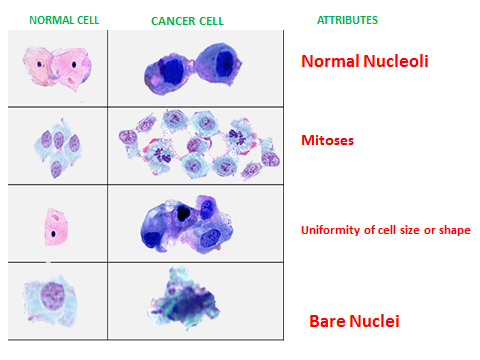
\includegraphics[scale=0.7]{attri}
\caption{normal vs cancerous cell attributes behavior}
\label{fig_attri}
\end{figure}

\subsection{Decision tree}
Decision tree is a popular classification method. Decision tree is used as a predictive model which maps observations about an item to conclusions about the item's target value. Rules produced by decision tree induction are easy to interpret and understand and hence can help greatly in appreciating the underlying mechanism that separate samples in different classes. One of the decision tree algorithms is c4.5. It builds decision trees from a set of training data using the concept of information entropy. It uses the information gain ratio criterion to determine the most discriminatory feature at each step of its  decision tree induction process. Pruning helps to reduce the size of decision trees by removing sections of the tree that provide little power to classify instances. Pruning reduces the complexity of the final classifier and hence improves predictive accuracy by the reduction of over fitting.
\begin{figure}[!h]
\centering
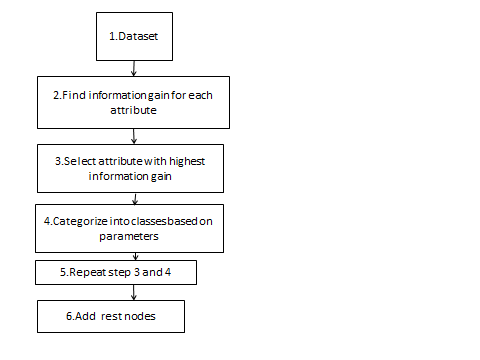
\includegraphics[scale=0.7]{c45bw}
\caption{Flowchart of C4.5}
\label{fig_sin}
\end{figure}
\\ \\
Algorithm:
\\Step 1: The leaf is labelled with the same class if the instances belong to the same class. \\
\\Step 2: For every attribute, the potential information will be calculated and the gain in information will be taken from the test on the attribute. \\
\\Step 3: Finally the best attribute will be selected based on the current selection parameter. \\


%\begin{equation}
$Entropy = - \sum_{i}p_{i} log_{2} p_{i}$
%\end{equation}
\\ \\
$Info(S)= - \sum_{i=1}^{k} \frac{freq (C_{i},S)}{|S|} log_{2}\frac{freq(C_{i},S)}{|S|}$
\\ \\where $Info(S)$ = entropy of sample training set $S$.
                        $C_{i}$ = class from 1 to n
Taken $ S=T$ 
\\ \\
$Info_{x}(T)=\sum_{i=1}^{n}((T_{i}/|T|)).Info(T_{i})$
\\
where $Info_{x}$ = entropy of each attribute
\\ \\ $T_{i}$ = subsets of samples from $1$ to $n$.
 \\ \\
$ \mbox{Information gain} (x)= Info(S) - Info_{x}(T)$


\subsection{Association Rules Mining}
Since its introduction in 1993 by Agarwal et. al.\cite{IEEEhowto:agarwal} the association rules mining has received a great amount of attention from several domains. Association Rules mining is the datamining process of finding the rules that may govern associations and causal objects between sets of items. It is used to find out association rules that satisfy the predefined minimum support and confidence from a given database. The problem is usually decomposed into two subproblems. One is to find those item sets whose occurrences exceed a predefined threshold in the database; those item sets are frequent or large item sets.The second problem is to generate association rules from those large item sets with the constriants of minimal confidence. One of the popular algorithms is the Aprioiri algorithm. It iteravely reduces the minimum support until it finds the required number of rules with the given minimum confidence.

The algorithm is designed to mine association rules. In general if  $\mbox{support}=freq(X,Y)/N$ and      $\mbox{confidence}=freq(X,Y)/freq(X)$  correspondingly then the rule is $X \rightarrow Y$, where $N$ is the no. of iterations.  For example: There is some database containing a set of attributes. The support and confidence is calculated and the rules generated can be seen. For example in figure \ref{fig_asso} there are 5 attributes going through 5 iterations. The rules generated are of the form $A \rightarrow D$ with support value of 0.4 and confidence value of 0.6. Similarly there can be more rules.
\begin{figure}[!h]
\centering
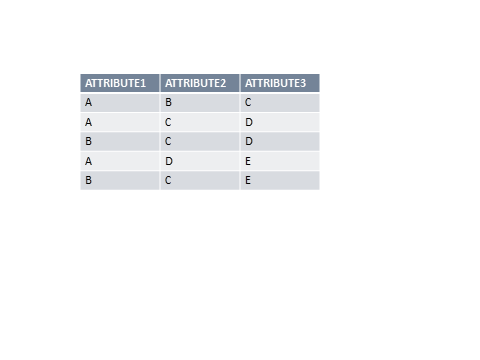
\includegraphics[scale=0.8]{asso}
\caption{Example-Association Rules Mining}
\label{fig_asso}
\end{figure}
 
% --------------------------------------------------------------------------------------------------------------------

 
%
\section{Proposed Model}
Fig \ref{fig_sin1} shows the functional block diagram of our proposed model. It consists of four steps: (a) Acquisition, (b) Preprocess, (c) Feature Selection and (d) Feature Extraction.
\begin{figure}[!h]
\centering
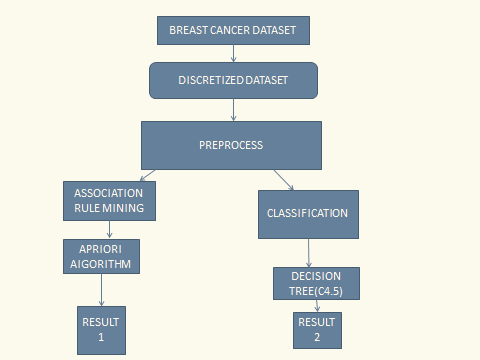
\includegraphics[scale=0.7]{PROPMODEL}
\caption{Proposed Model}
\label{fig_sin1}
\end{figure}

In acquisition step, we get the dataset. In our work here we have clinical records for cancerous cell. Then in preprocessing we prepare the data to fit with several data mining techniques. These Data Mining techniques guide us to select the suitable features and extract these for the purpose of classification of benign and malignant cases. In figure \ref{fig_sin1}  we first discretize the dataset for generating nominal values, then pre-process the data to eliminate incomplete information. Thereafter we adopt two Data Mining techniques namely, Association Rules Mining using Apriori Algorithms and classification using Decision Tree and come with respective results as shown in figure \ref{fig_sin1}. This guides the doctors to consider appropriate therapy as an automatic support tool during their treatment.

\section{Methodology}
The attributes of the dataset are found as listed in Table 1.
\vspace{.3 cm}

 \begin{center}
     \textbf{Table1: WISCONSIN BREAST CANCER DATASET ATTRIBUTES}
  \end{center}

    \begin{tabular}{|c|c|c|}
      \hline
      & Attribute & Domain\\
      \hline
      1 & Sample Code No & id no\\
      \hline
      2 & Clump Thickness & 1-10\\
      \hline
      3 & Uniformity(Cell Size) & 1-10\\
      \hline
      4 & Uniformity(Cell Shape) & 1-10\\
       \hline
      5 & Marginal Adhesion & 1-10\\
       \hline
      6 & sgl Epithelial(cell size) & 1-10\\
       \hline
      7 & Bare Nuclei & 1-10\\
       \hline
      8  & Bland Chromatin & 1-10\\
       \hline
      9 & Normal Nucleoli & 1-10\\
       \hline
      10 & Mitoses & 1-10\\
       \hline
      11 & Class & 2 or 4\\
      \hline
    \end{tabular}

\vspace{.5 cm}
In the Clump thickness benign cells tend to be grouped in monolayers, while cancerous cells are often grouped in multilayers. While in the Uniformity of cell size/shape the cancer cells tend to vary in size and shape. That is why these parameters are valuable in determining whether the cells are cancerous or not. In the case of Marginal adhesion the normal cells tend to stick together, where cancer cells tend to lose this ability. So loss of adhesion is a sign of malignancy. In the Single epithelial cell size the size is related to the uniformity
mentioned above. Epithelial cells that are significantly enlarged may be a malignant cell. The Bare nuclei is a term used for nuclei that is not surrounded by cytoplasm (the rest of the cell). Those are typically seen in benign tumors. The Bland Chromatin describes a uniform "texture" of the nucleus seen in benign cells. In cancer cells the chromatin tends to be coarser. The Normal nucleoli are small structures seen in the nucleus. In normal cells the nucleolus is usually very small if visible. In cancer cells the nucleoli become more prominent, and sometimes there are more of them. Finally, Mitoses is nuclear division plus cytokines and produce two identical daughter cells during prophase. It is the process in which the cell divides and replicates. Pathologists can determine the grade of cancer by counting the number of mitoses cell division.


We next present our algorithm and further describe the dataset on which we have evaluated. Our first step is to discretize the dataset into three major groups.

\begin{enumerate}
\item Low
\item Mid
\item High
\end{enumerate}

\begin{algorithm}[H]
\caption{An algorithm for discretization  of dataset}


\textbf{Input} : Dataset in excel format with $9$ parameters.

\textbf{Output:} : Dataset in csv file (space delimiter) format in discrete format with all $9$ parameters.

\textbf{Algorithmic Steps:}
\begin{enumerate}
  \item Obtain the ranges of high, middle and low.
  \item Collect every cell value for computation for every parameter.
  \item \textbf{For} parameter $1$ to $9$ do
  \item \textbf{If} Cell value $>$= high value \textbf{Then}
            \textbf{Put} new Cell value= 'H'
            \textbf{Else If} Cell value $>$= middle value \textbf{Then}
             \textbf{Put} new Cell value= 'M'
             \textbf{Else}
             \textbf{Put} new Cell value= 'L'
  \item \textbf{End if}
  \item \textbf{Next}
  \item \textbf{For} $10^{th}$ parameter
  \item \textbf{If} Cell value = 2 \textbf{Then}
  \item \textbf{Put} new Cell value = "Benign"
  \item \textbf{Else If} Cell value = 4 then
  \item \textbf{Put} new Cell value = "Malignant"
  \item \textbf{End If}
  \item Construct another excel file based on this discrete value.
  \item Convert the excel file into csv(space delimiter) file.
\end{enumerate}

\end{algorithm}



As the parameter of the dataset ranges from 1 to 10 we made this discretization based on different ranges like:-

\begin{enumerate}
\item low:- 1 to 1, mid:- 2 to 6, high:- 7 to 10
\item low:- 1 to 1, mid:- 2 to 7, high:- 8 to 10
\item low:- 1 to 2, mid:- 3 to 7, high:- 8 to 10
\item low:- 1 to 3, mid:- 4 to 6, high:- 7 to 10
\item low:- 1 to 4, mid:- 5 to 6, high:- 7 to 10
\item low:- 1 to 4, mid:- 5 to 7, high:- 8 to 10
\end{enumerate}

 --------------------------------------------------------------------------------------------------------------------





% --------------------------------------------------------------------------------------------------------------------
 --------------------------------------------------------------------------------------------------------------------
\section{Results}


Based on these cell's behavior the dataset's attributes values can largely help in determination and diagnosis. On discretisation and preprocessing, each attribute shows its own graphical result divided into 3 categories based on high, medium and low values. 

\begin{figure}[!h]
\centering
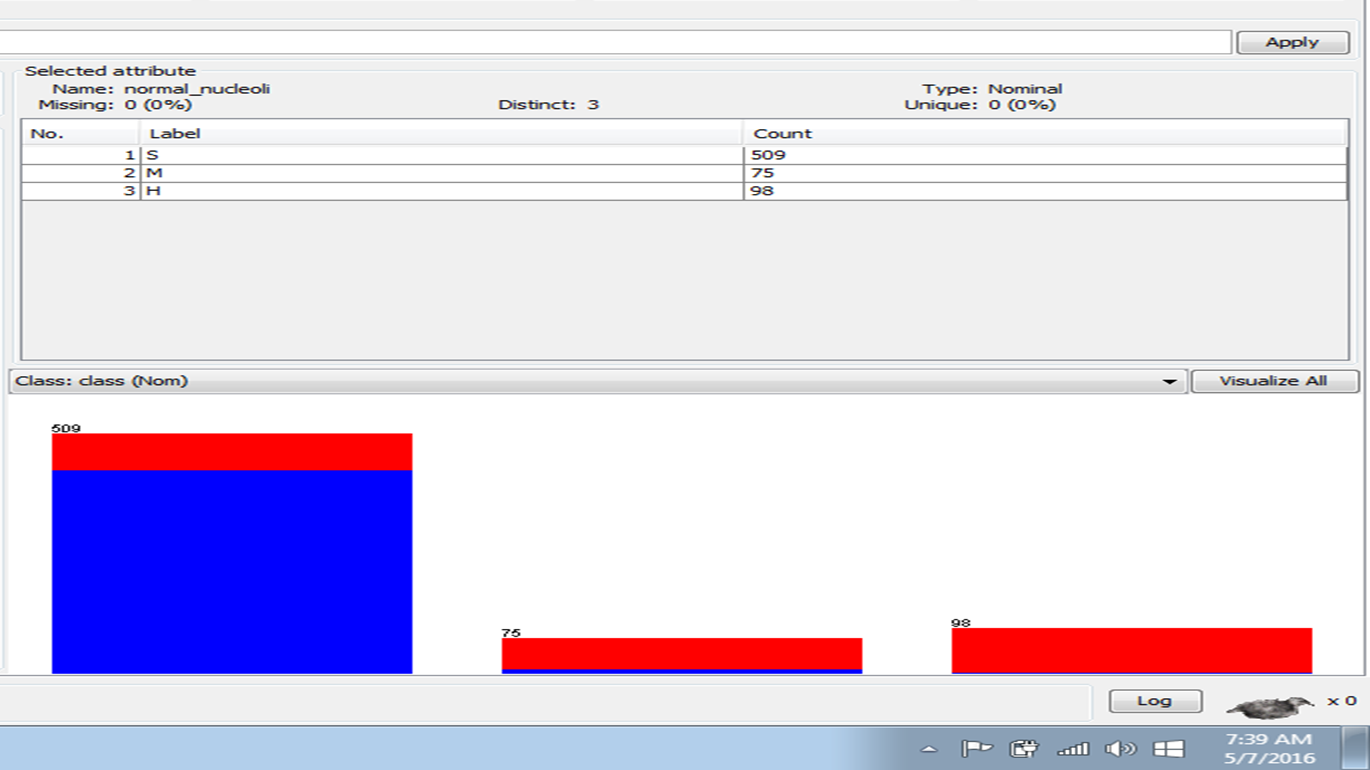
\includegraphics[scale=0.32]{nucleifig}
\caption{normal nucleoli}
\label{fig_nucle}

\end{figure}

Figure \ref{fig_nucle}  shows normal nucleoli attribute and the no. of patient instances classified into benign and malignant group. The figure shows that out of 509 instances with low or small value has 30\% malignant and 70\% benign then out of 75 instances with medium value 90\% are Malignant and 10\% Benign then out of 98 instances with high value 99\% are Malignant and 1\% benign cases.

The overall result is further shown in Figure \ref{fig_tree} in the form of a Decision tree (Also known as J48 pruned tree). The detail of this observed result in WEKA platform classifies the Benign (non-cancerous) and Malignant (cancerous) classes based on selected cell attributes (e.g., size uniformity, Bare nuclei, Bland Chromatin and Shape uniformity) as shown in this figure. According to the observation  the higher the value of the attributes the greater the tendency towards malignancy.On observing the J48 pruned tree and considering only the malignant category we can see that a combination of two medium values or one high and another medium value or only high values can help in determining the malignancy.
 

%Similarly all attributes can be visualised at a time shown in figure below. 
%\begin{figure}[!h]
%\centering
%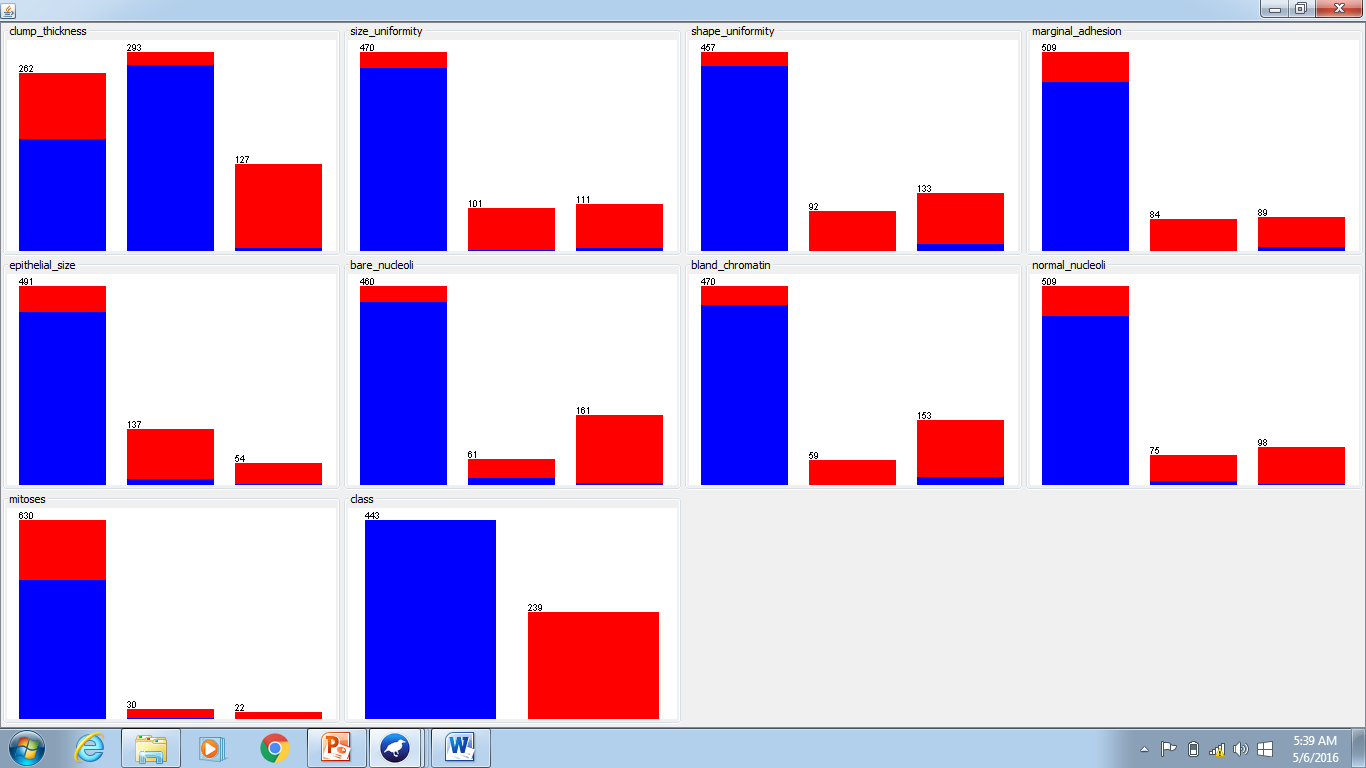
\includegraphics[scale=0.3]{visuals}
%\caption{All attributes}
%\label{fig_sin}
%
%\end{figure}



\begin{figure}[!h]
\centering
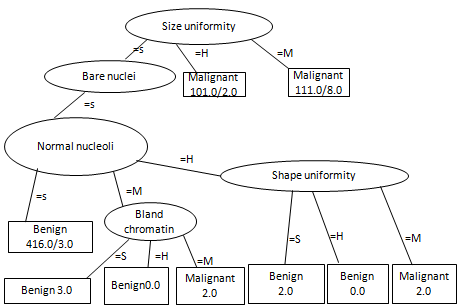
\includegraphics[scale=0.5]{tree}
\caption{Decision tree (J48 pruned tree)}
\label{fig_tree}
\end{figure}


%benign.
Also we have applied this modified dataset in WEKA Tool for further analysis; and we got the following results:


\begin{enumerate}
  \item We observe that the value of Clump Thickness \& Bare Nucleoli tends to be in higher side. More than $20\%$ of the values are in higher side, compare to other parameters who ranges on $16\%$ in higher side.

  \item More than $35\%$ of the value for the parameter Clump thickness, Epithelial size \& bland chromatin ranges in medium side.

  \item Bare Nucleoli's medium range value is in $< 11\%$ data whereas others had an average of $20\%$.

  \item Malignancy is positive when Clump Thickness \& Bare Nucleoli is in higher side but Size Uniformity \& Shape Uniformity has a very sensitive effect, i.e when the value is $>=4$ there shows a positive sign of malignancy in more than $80\%$ cases.

  \item More than $64\%$ malignancy is positive only due to these two parameters.

  \item For marginal adhesion \& epithelial size, value ranges between $2$ to $5$. More than $40\%$ cases it is malignancy when this two parameter is low.

  \item In case of Bare Nucleoli \& Normal Nucleoli, in $70\%$ cases they tends to be low. They also show positive malignancy in $40\%$ cases when they are low. They have $60\%$ values in between $3$ to $4$. If the value is $5$ or more then definitely it is malignancy.
\end{enumerate}

Selection of the most useful attribute is necessary. Information gain evaluator can help to find the attribute highest priority. The output presented  in figure \ref{fig_rank} shows information gain values of each and every attribute and their ranking. Size uniformity is selected as the best one. Then shape uniformity taken into consideration. On selecting a set of attributes based on the ranking we get one or different kinds of rules. Among them the best and of utmost importance are selected.

\begin{figure}[!h]
\centering
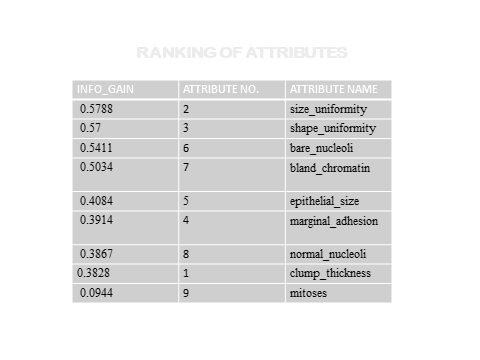
\includegraphics[scale=0.7]{RANKING}
\caption{Ranking of attributes}
\label{fig_rank}
\end{figure}
Figure \ref{fig_asorules}  shows the different association rules generated using  uniformity of size,uniformity of shape  and class after applying the Apriori algorithm. Among them rules no.2,3,4, 13 give significant results for determining malignancy.
The first rule says that when there are 425 instances with uniformity of shape value to be small and the class they belong to is benign then 424 instances with small valued size uniformity attribute also follows showing confidence as 1.This rule does not seem to be so interesting to determine malignancy. Therefore on further analyzing it is  found that rule no.2,3,4 and 13 gives some thoughtful and result oriented knowledge.
The second rule says that 92 instances with  high value in shape-uniformity leads to malignant class with confidence of 0.99
The third rule says that 73 high valued instances in both size-uniformity shape-uniformity leads to class malignant consisting 72 instances having confidence of 0.99.
The fourth rule says that 101 instances with high valued size-uniformity is followed by 99 instances falling in malignant class showing confidence of 0.98.
The thirteenth rule says that 111 instances with size-uniformity value as medium is followed by malignant class with 103 instances having confidence 0.93.

\begin{figure}[!h]
\centering
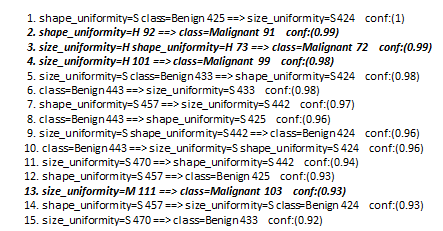
\includegraphics[scale=0.7]{asorules}
\caption{Association Rules}
\label{fig_asorules}
\end{figure}



 The results as shown in Figure \ref{fig_class} shown the  different statistical measures, like Kappa statistics, mean absolute error and all the other parameters (as shown in figure \ref{fig_class} ) have their own significance and importance.

\begin{figure}[!h]
\centering
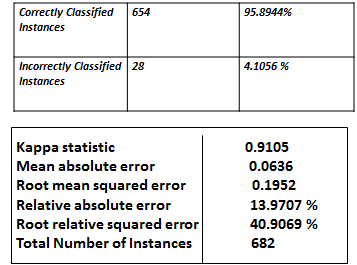
\includegraphics[scale=0.7]{classification}
\caption{classification results}
\label{fig_class}
\end{figure}

As an example by studying these measure, the argument between two or more observers that taken into account the fact that observers will sometimes agree or disagree simply by chance.The calculation is based on the difference between how much agreement is actually present (observed agreement) compared to how much agreement would be expected to be  present by chance alone (expected agreement).The Mean Absolute Error (MAE) and Root Mean Square Error (RMSE) can be used together to diagnose the variation in the errors in a set of forecasts. The RMSE will always be larger or equal to the MAE; The greater the difference between them  the greater the variance in the individual errors in the sample. If RMSE=MAE then all the errors are of the same magnitude.

\begin{figure}[!h]
\centering
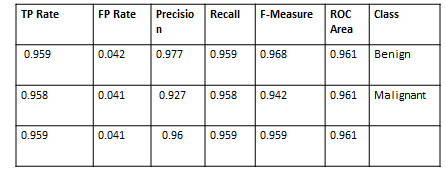
\includegraphics[scale=0.7]{accuracy}
\caption{Accuracy Measures}
\label{fig_accuracy}
\end{figure}
The figure \ref{fig_accuracy} shows the detailed accuracy result with the help of some terms as True positive rate,False positive rate etc.The last row in the table gives the weighted average among the found result. 


In the figure \ref{fig_confusion} rows show the actual instances and the column shows the predicted instances. a means benign and b means malignant. \\The result shows that
 425 instances are actually benign and predicted benign (True Positive).
\\18 instances are actually benign but predicted malignant (False Negative).
\\10 instances are actually malignant but predicted benign (False Positive).
\\229 instances are actually malignant and predicted malignant (True Negative).

\begin{figure}[!h]
\centering
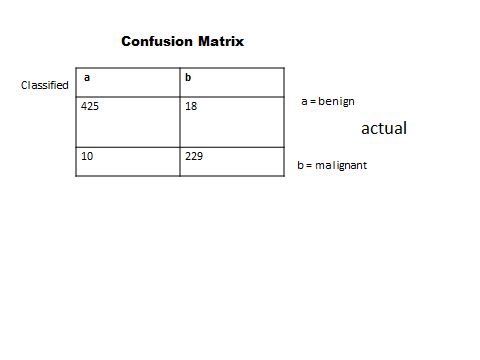
\includegraphics[scale=0.7]{confusion}
\caption{Resultant confusion matrix}
\label{fig_confusion}
\end{figure}

% An example of a floating figure using the graphicx package.
% Note that \label must occur AFTER (or within) \caption.
% For figures, \caption should occur after the \includegraphics.
% Note that IEEEtran v1.7 and later has special internal code that
% is designed to preserve the operation of \label within \caption
% even when the captionsoff option is in effect. However, because
% of issues like this, it may be the safest practice to put all your
% \label just after \caption rather than within \caption{}.
%
% Reminder: the "draftcls" or "draftclsnofoot", not "draft", class
% option should be used if it is desired that the figures are to be
% displayed while in draft mode.
%
%\begin{figure}[!t]
%\centering
%\includegraphics[width=2.5in]{myfigure}
% where an .eps filename suffix will be assumed under latex, 
% and a .pdf suffix will be assumed for pdflatex; or what has been declared
% via \DeclareGraphicsExtensions.
%\caption{Simulation results for the network.}
%\label{fig_sim}
%\end{figure}

% Note that the IEEE typically puts floats only at the top, even when this
% results in a large percentage of a column being occupied by floats.


% An example of a double column floating figure using two subfigures.
% (The subfig.sty package must be loaded for this to work.)
% The subfigure \label commands are set within each subfloat command,
% and the \label for the overall figure must come after \caption.
% \hfil is used as a separator to get equal spacing.
% Watch out that the combined width of all the subfigures on a 
% line do not exceed the text width or a line break will occur.
%
%\begin{figure*}[!t]
%\centering
%\subfloat[Case I]{\includegraphics[width=2.5in]{box}%
%\label{fig_first_case}}
%\hfil
%\subfloat[Case II]{\includegraphics[width=2.5in]{box}%
%\label{fig_second_case}}
%\caption{Simulation results for the network.}
%\label{fig_sim}
%\end{figure*}
%
% Note that often IEEE papers with subfigures do not employ subfigure
% captions (using the optional argument to \subfloat[]), but instead will
% reference/describe all of them (a), (b), etc., within the main caption.
% Be aware that for subfig.sty to generate the (a), (b), etc., subfigure
% labels, the optional argument to \subfloat must be present. If a
% subcaption is not desired, just leave its contents blank,
% e.g., \subfloat[].


% An example of a floating table. Note that, for IEEE style tables, the
% \caption command should come BEFORE the table and, given that table
% captions serve much like titles, are usually capitalized except for words
% such as a, an, and, as, at, but, by, for, in, nor, of, on, or, the, to
% and up, which are usually not capitalized unless they are the first or
% last word of the caption. Table text will default to \footnotesize as
% the IEEE normally uses this smaller font for tables.
% The \label must come after \caption as always.
%
%\begin{table}[!t]
%% increase table row spacing, adjust to taste
%\renewcommand{\arraystretch}{1.3}
% if using array.sty, it might be a good idea to tweak the value of
% \extrarowheight as needed to properly center the text within the cells
%\caption{An Example of a Table}
%\label{table_example}
%\centering
%% Some packages, such as MDW tools, offer better commands for making tables
%% than the plain LaTeX2e tabular which is used here.
%\begin{tabular}{|c||c|}
%\hline
%One & Two\\
%\hline
%Three & Four\\
%\hline
%\end{tabular}
%\end{table}


% Note that the IEEE does not put floats in the very first column
% - or typically anywhere on the first page for that matter. Also,
% in-text middle ("here") positioning is typically not used, but it
% is allowed and encouraged for Computer Society conferences (but
% not Computer Society journals). Most IEEE journals/conferences use
% top floats exclusively. 
% Note that, LaTeX2e, unlike IEEE journals/conferences, places
% footnotes above bottom floats. This can be corrected via the
% \fnbelowfloat command of the stfloats package.




\section{Conclusion}
In this paper we have addressed the problem of breast cancer treatment. As the granularity of cases is robust,  here we adapt the advantages of Data Mining techniques to build a Decision support systems for practitioners. Here in particular we consider two Data Mining techniques, namely Decision tree and Association rules mining.We noticed that during the analysis of cell centric information of cancerous and non-cancerous cases, we get some results which encourage us to come with an automated Decision support system for therapy. As the analysis is very much data centric, the variation of clinical data/ diagnostic information can vary the outcome. Some more Data Mining techniques could be adapted for future study and improvement of the result. Also we are considering the  comparative analysis  of the existing results with our achieved result.





% conference papers do not normally have an appendix


% use section* for acknowledgment
%\section*{Acknowledgment}
%
%
%The authors would like to thank...





% trigger a \newpage just before the given reference
% number - used to balance the columns on the last page
% adjust value as needed - may need to be readjusted if
% the document is modified later
%\IEEEtriggeratref{8}
% The "triggered" command can be changed if desired:
%\IEEEtriggercmd{\enlargethispage{-5in}}

% references section

% can use a bibliography generated by BibTeX as a .bbl file
% BibTeX documentation can be easily obtained at:
% http://mirror.ctan.org/biblio/bibtex/contrib/doc/
% The IEEEtran BibTeX style support page is at:
% http://www.michaelshell.org/tex/ieeetran/bibtex/
%\bibliographystyle{IEEEtran}
% argument is your BibTeX string definitions and bibliography database(s)
%\bibliography{IEEEabrv,../bib/paper}
%
% <OR> manually copy in the resultant .bbl file
% set second argument of \begin to the number of references
% (used to reserve space for the reference number labels box)
\begin{thebibliography}{1}

%\bibitem{IEEEhowto:kopka}
%H.~Kopka and P.~W. Daly, \emph{A Guide to \LaTeX}, 3rd~ed.\hskip 1em plus
%  0.5em minus 0.4em\relax Harlow, England: Addison-Wesley, 1999.

\bibitem{IEEEhowto:agarwal}
Agarwal,~R., Imielinski,~ T., and Swami, ~A. N. ,1993. \emph{ Mining association rules 
between sets of items in large databases.  } \hskip 1em plus
  0.5em minus 0.4em\relax In Proceedings of the 1993 ACM SIGMOD International Conference on Management of Data, 207-216.

\bibitem{IEEEhowto:delen}
Delen ~D, Patil ~N, \emph{Knowledge extraction from prostate cancer data}.\hskip 1em plus
  0.5em minus 0.4em\relax. The 39thAnnual Hawaii International Conference on System Sciences; 2006; 1-10.

  \bibitem{IEEEhowto:nci}
National Cancer Institute, \emph{Surveillance, Epidemiology, and End Results (SEER) Program Public-Use Data (1973-2008).}\hskip 1em plus
  0.5em minus 0.4em\relax Cancer Statistics Branch; 2011.
  
  \bibitem{IEEEhowto:elsayad}
A.M.~Elsayad and H.A.~Elsalamony. , \emph{Diagnosis of Breast Cancer using Decision Tree Models and SVM}, \hskip 1em plus
  0.5em minus 0.4em\relax International Journal of Computer Application (0975-8887),Volume 83-No 5,December 2013
  
   \bibitem{IEEEhowto:ahmed}
Ahmad~LG, Eshlaghy~AT, Poorebrahimi~A, Ebrahimi~M and Razavi~AR , \emph{Using three machine learning techniques for predicting Breast cancer recurrence }, \hskip 1em plus
  0.5em minus 0.4em\relax Health Med Inform 2013,4:2.
  
  \bibitem{IEEEhowto:shajahaan}
S.S.~Shajahaan, S.~Shanthi, V. ~Mano Chitra, \emph{Application of Data Mining Techniques to Model Breast Cancer Data.},.\hskip 1em plus 0.5em minus 0.4em\relax . International Journal of Emerging Technology And Advanced Engineering, ISSN 2250-2459,ISO 9001:2008 Certified Journal, Volume 3,Issue 11,November 2013.

   \bibitem{IEEEhowto:samar}
Samar Al-Qarzaie, Sara Al –Odhaibi, Bedoor Al-Saeed and Dr. Mohammed Al-Hagery.  , \emph{Using the Data Mining Techniques for Breast Cancer Early Prediction }, \hskip 1em plus
  0.5em minus 0.4em\relax 2013
  
  \bibitem{IEEEhowto:chaurasia}
  V.~Chaurasia and S.~Pal., \emph{ Data Mining Techniques: To predict and resolve breast cancer survivabilty.}, \hskip 1em plus
  0.5em minus 0.4em\relax International Journal of Computer Science and Mobile Computing,vol.3 Issue 1, January-2014

   \bibitem{IEEEhowto:uci}
UCI machine Learning Repository, \emph{http://archive.ics.uci.edu/ml/ }, \hskip 1em plus 0.5em minus 0.4em\relax 

%  \bibitem{IEEEhowto:kopka}
%www.komen.org/risk \emph{ } \hskip 1em plus 0.5em minus 0.4em\relax 

\bibitem{IEEEhowto:bellaachia}
   A.~Bellaachia and Erhan ~Guven., \emph{Predicting Breast Cancer Survivability using Data Mining Techniques.}, \hskip 1em plus
  0.5em minus 0.4em\relax Dept.of Computer Science, The George Washington University. Washington DC 20052  
  
  \bibitem{IEEEhowto:ahmed}
 Kawsar Ahmed, Abdullah –Al-Emran, Tasnuma Jesmin, Roshney Fatima Mukti, Md Zamilur Rahman and Farzana Ahmed\emph{Early detection of lung cancer risk using Data Mining.} \hskip 1em plus  0.5em minus 0.4em\relax DOI:http://dx.doi.org/10.7314/APJCP .2013.14.1.595
   
  \bibitem{IEEEhowto:soni}
  Jyoti Soni, Ujma Ansari , Dipesh Sharma and Sunita Soni\emph{Predictive Data Mining for Medical Diagnosis: An Overview of Heart Disease Prediction.} \hskip 1em plus
  0.5em minus 0.4em\relax International   Journal of Computer Applications (0975 – 8887) Volume 17– No.8, March 2011
  
 \bibitem{IEEEhowto:thazin}
Htet Thazin, Tike Thein1 and Khin Mo Mo Tun2,   \emph{ Department of Computational Mathematics, University of Computer Studies, Yangon,Myanmar. An approach for breast cancer diagnosis classification using neural network.}, \hskip 1em plus 0.5em minus 0.4em\relax Advanced Computing: An International Journal (ACIJ), Vol.6, No.1, January 2015
   
 \bibitem{IEEEhowto:tzanis}
George ~Tzanis, Christos ~Berberidis, and Ioannis ~Vlahavas,\emph{Biological Data Mining }, \hskip 1em plus 0.5em minus 0.4em\relax   Department of  Informatics, Aristotle University of Thessaoniki, Greece
  
\bibitem{IEEEhowto:thangaraju}
Thangaraju ~P1, Barkavi ~G2, Karthikeyan ~.T, \emph{ Mining Lung Cancer Data for Smokers and Non-Smokers by Using Data Mining Techniques }, \hskip 1em plus 0.5em minus 0.4em\relax International Journal of Advanced Research in Computer and Communication Engineering Vol. 3, Issue 7, July 2014

\bibitem{IEEEhowto:lavanya}
  D.~Lavanya and Dr.K.~Usha Rani. \emph{ Ensemble decision tree classifier for breast cancer data.} \hskip 1em plus 0.5em minus 0.4em\relax  International Journal of Information Technology Convergence and Services (IJITCS) Vol.2, No.1, February 2012
  
  \bibitem{IEEEhowto:patel}
  Neha ~Patel and  Divakar ~Singh.\emph{ An Algorithm to Construct Decision Tree for Machine Learning based on Similarity Factor.}, \hskip 1em plus
  0.5em minus 0.4em\relax International Journal of Computer Ap-plications (0975 – 8887) Volume 111 – No 10, February 2015
  
 \bibitem{IEEEhowto:ruggieri}
   Salvatore Ruggieri,\emph{Efficient C4.5.Dipartimento di Informatica}, \hskip 1em plus 0.5em minus 0.4em\relax Universita di Pisa Corso Italia 40, 56125 Pisa Italy

   
\bibitem{IEEEhowto:tyrer}
 Jonathan Tyrer, Stephen W. Duffy and Jack Cuzick. \emph{A breast cancer prediction model incorporating familial and personal risk factors}, \hskip 1em plus
  0.5em minus 0.4em\relax Department of Epidemiology; Mathematics and Statistics; Cancer Research U.K.; Wolfson Institute of Preventive Medicine; Charterhouse Square; London EC1M 6BQ; U.K.  STATISTICS IN MEDI-CINE Statist. Med. 2004; 23:1111–1130 (DOI: 10.1002/sim.1668)

\end{thebibliography}




% that's all folks
\end{document}


